\section{Visual Design}
In order to generate a visual design for the application, the psychological effects of perception must be taken into accountt as a core aspect. The graphical user interface (GUI) is essential since the credibility judgments of a user over an website or application are based about 75\% on its aesthetics and occur in less than 3.5 seconds \parencite[cf.][1]{Alsudani.2009}.
\subsection{Psychology of Perception}
\paragraph*{} Those principles help developers to improve the structural and content wise design of their application, and - as it simplifies the understandability of the application - also the perception of the user, but aesthetic are not directly touched by these. The Gestalt theory describes eight laws for aesthetic designs, which relate to the principle of \textit{Exploiting Prior Knowledge} in terms of using intuitive perceptions of human brains to visually group objects to create a visual composition \parencite[cf.][113]{Sternberg.2012}.
\begin{enumerate}
    \item \textbf{Law of Proximity:} Objects that are close to each other, are perceived as mate (cf. \Cref{fig:prox}). For things to be relatively close to each other, groups must be separated by a larger white space. \parencite{Seogaard.n.y.}
    \item \textbf{Law of Similarity:} As to be seen in \Cref{fig:sim}, objects that share visual properties group themselves visually \parencite[cf.][2]{Bakar.2017}.
    \begin{figure}[H] 
        \begin{minipage}[b]{.5\linewidth}
            \centering
\includegraphics[width=0.94\textwidth]{img/proximity.pdf}
            \subcaption{proximity}\label{fig:prox}
        \end{minipage}%
        \begin{minipage}[b]{.5\linewidth}
            \centering
\includegraphics[width=0.94\textwidth]{img/similarity.pdf}
            \subcaption{similarity}\label{fig:sim}
        \end{minipage}
        \caption[Laws of Proximity and Similarity]{Examples of the laws of proximity and similarity (own illustrations)}\label{fig:law1}
    \end{figure}
    \item \textbf{Law of Closure:} Objects that are grouped by visual perception (e.g. by proximity or symmetry) are experienced as a whole (cf. \Cref{fig:sym}). This principle may suggest objects that are none-existent on the interface \parencite[cf.][]{Stevenson.n.y.}.
    \item \textbf{Law of Symmetry:} Humans tend to perceive objects as two approximate symmetrical halves wherever possible; separate symmetric objects are therefore more likely to be perceived as being one coherent object \parencite[cf.][]{Soegaard.n.y.}.
    \begin{figure}[H] 
        \begin{minipage}[b]{.5\linewidth}
            \centering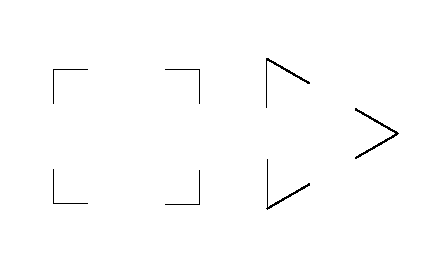
\includegraphics[width=0.94\textwidth]{img/closure.pdf}
            \subcaption{closure}\label{fig:clo}
        \end{minipage}%
        \begin{minipage}[b]{.5\linewidth}
            \centering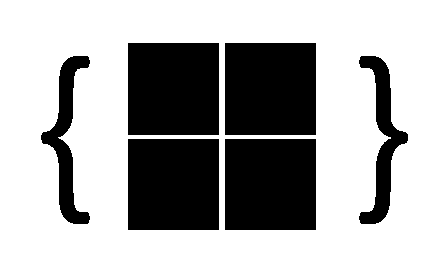
\includegraphics[width=0.94\textwidth]{img/symmetry.pdf}
            \subcaption{symmetry}\label{fig:sym}
        \end{minipage}
        \caption[Laws of Closure and Symmetry]{Examples of the laws of closure and symmetry (own illustrations)}\label{fig:law2}
    \end{figure}
    \item \textbf{Law of Common Fate:} Objects that are moving in the same direction are visually connected, while separating those fixed in position or moving differently \parencite{Todorovic.2008}.
    \item \textbf{Law of Continuity:} Visual perception prefers to follow smooth lines. This may result in misleading predictions and a tendency to find smooth continuation more favorable than rough ones, but can also suggest users to follow a certain path of looking or navigating. \parencites{Bakar.2017}{Todorovic.2008}
    \begin{figure}[H] 
        \begin{minipage}[b]{.5\linewidth}
            \centering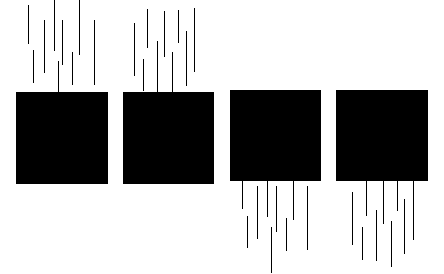
\includegraphics[width=0.94\textwidth]{img/fate.pdf}
            \subcaption{common fate}\label{fig:fate}
        \end{minipage}%
        \begin{minipage}[b]{.5\linewidth}
            \centering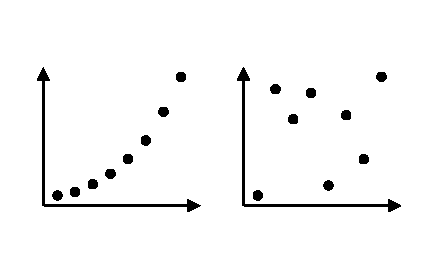
\includegraphics[width=0.94\textwidth]{img/continuity.pdf}
            \subcaption{continuity}\label{fig:con}
        \end{minipage}
        \caption[Laws of Common Fate and Continuity]{Examples of the laws of common fate and continuity (own illustrations)}\label{fig:law3}
    \end{figure}
    \item \textbf{Law of Good Gestalt:} Groups with regular patterns are more easily perceived and remembered than unstructured ones, because two different patterns within one group, instinctively separates the group into two, as it can be seen in \Cref{fig:gest} \parencite{Todorovic.2008}.
    \item \textbf{Law of Past Experience:} Sometimes also named \textit{Law of Pragnance}, the law of past experience is the risk of a human to filter out information and reducing the perceived information to more common examples \parencite{Stevenson.n.y.}. In \Cref{fig:exo} an capital ''L'' and ''I'' will form a capital ''U'' in perveption, which may not be the implicated goal. On the other hand one can use that profitable as the emoticon is a common way to express sentiment in short form.
    \begin{figure}[H] 
        \begin{minipage}[b]{.5\linewidth}
            \centering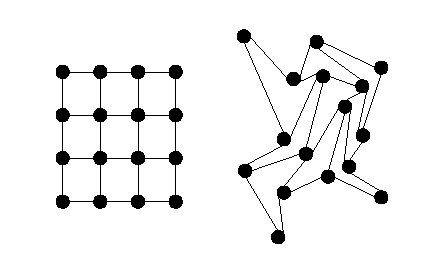
\includegraphics[width=0.94\textwidth]{img/gestalt.pdf}
            \subcaption{good gestalt}\label{fig:gest}
        \end{minipage}%
        \begin{minipage}[b]{.5\linewidth}
            \centering
\includegraphics[width=0.94\textwidth]{img/experience.pdf}
            \subcaption{past experience}\label{fig:exo}
        \end{minipage}
        \caption[Laws of Good Gestalt and Past Experience]{Examples of the laws of good gestalt and past experience (own illustrations)}\label{fig:law4}
    \end{figure}
\end{enumerate}
\subsection{Attention Economy}
Attention economy deals with the scarcity of the ability of people to pay attention. In modern times, one does not only do one thing at work, but is continuously given information  \parencite[cf.][]{Davenport.2001}. \textcite{Davenport.2001} state, that for successful transfer of knowledge, understanding attention economy is essential. 
\paragraph*{} The attention of people is treated as a limited resource in the concept of attention economy. It is distinguished by the trait of being naturally limited and transient. This means, that a moment not used for paying attention for something is neither able to be restored nor savable. \parencite[cf.][]{Davenport.2001}
\paragraph*{} The reason for attention economy to become relevant is the increasing amount of available information. The increasing diversity and density of information caused in the mainstream of digital media and the internet in form of online news, e-mail, social media etc. in addition to traditional communication and information channels such as TV, radio, telephony, letters etc.
\paragraph*{} Derived from that, one can regard attention as a money worth good \parencite[cf.][]{Davenport.2001}. While market penetration is narrative for marketing purposes, one must take into account, that potential users of a application may leave it after a short period of time in favor of competing consumers of attention. Designing user interfaces to keep the users attention, and winning it back later is key for getting the marketing idea and the implication of attention economy together.
